% \documentclass[aspectratio=169]{beamer} % 16:9 aspect ratio for modern screen
\documentclass[handout]{beamer} % 16:9 aspect ratio for modern screen

% Theme settings
\usetheme[progressbar=foot]{metropolis} % Minimalist theme
\metroset{progressbar=frametitle} % Progress bar soll nur folien mit titel berücksichtigen?
\setbeamercolor{background canvas}{bg=white} % White background color

\makeatletter
    \setlength{\metropolis@progressinheadfoot@linewidth}{1.5pt}
\makeatother


\usefonttheme{professionalfonts} % Font theme

% Packages
\usepackage[T1]{fontenc}   % Font encoding
\usepackage[ngerman]{babel} % German language
\usepackage[sfdefault]{FiraSans} % For FiraSans font
\usepackage[backend=biber, style=authoryear-comp
, sorting=nyt]{biblatex} % For bibliography
\usepackage{csquotes} % Recommended for biblatex with babel/polyglossia
\usepackage{textgreek} % Greek letters in text mode (aus references von Citavi)
\usepackage{tikz}          % For drawing graphics

\usepackage{graphicx}       % For including images
\usepackage{amsmath, amssymb} % For math symbols

\usepackage[labelformat=empty]{caption}


% Bibliography settings
\addbibresource{references.bib} % Path to the bibliography file

% custom Citation commands
\DeclareCiteCommand{\citeauthortitle}
  {\usebibmacro{prenote}}
  {\usebibmacro{citeindex}%
   \printnames{labelname}%
   \setunit{\space\textendash\space}
   \printfield{title}}
  {\multicitedelim}
  {\usebibmacro{postnote}}

  \DeclareCiteCommand{\citeauthortitleurl}
  {\usebibmacro{prenote}}
  {\usebibmacro{citeindex}%
   \printnames{labelname}%
   \setunit{\space\textendash\space}
   \printfield{title}%
   \setunit{\addsemicolon\space}
   \printfield{url}}
  {\multicitedelim}
  {\usebibmacro{postnote}}

\DeclareCiteCommand{\parenciteauthortitle}
  {\usebibmacro{prenote}}
  {\bibopenparen\usebibmacro{citeindex}%
   \printnames{labelname}%
   \setunit{\space\textendash\space}% <- Hier wird das Trennzeichen ":" hinzugefügt
   \printfield{title}\bibcloseparen}
  {\multicitedelim}
  {\usebibmacro{postnote}}

\makeatletter
\renewcommand\footnotesize{\tiny}
\makeatother

\newcommand{\figcite}[1]{\\[-3mm]{\tiny Quelle: \cite{#1}}}
\newcommand{\figciteweb}[1]{\\[-3mm]{\tiny aus: \citeauthortitle{#1}}}
\newcommand{\figciteweburl}[1]{\\[-3mm]{\tiny aus: \citeauthortitleurl{#1}}}
  
\mode<handout>{
    \AtBeginSection[]{} % In Handout-Version keine Section-Folie erzeugen
}

% Title page settings
\title{Presentation Title}
\subtitle{Subtitle of the Presentation}
\author{Florian Adamczyk}
\date{\today}

\begin{document}

    % Black slide
    \begin{frame}<handout:0>[plain, noframenumbering]
        \begin{tikzpicture}[remember picture, overlay]
            \fill[black] (current page.south west) rectangle (current page.north east);
        \end{tikzpicture}
    \end{frame}

    % Appetizer Slide
    \begin{frame}<handout:0>[noframenumbering, plain]{Appetizer}
        \centering
        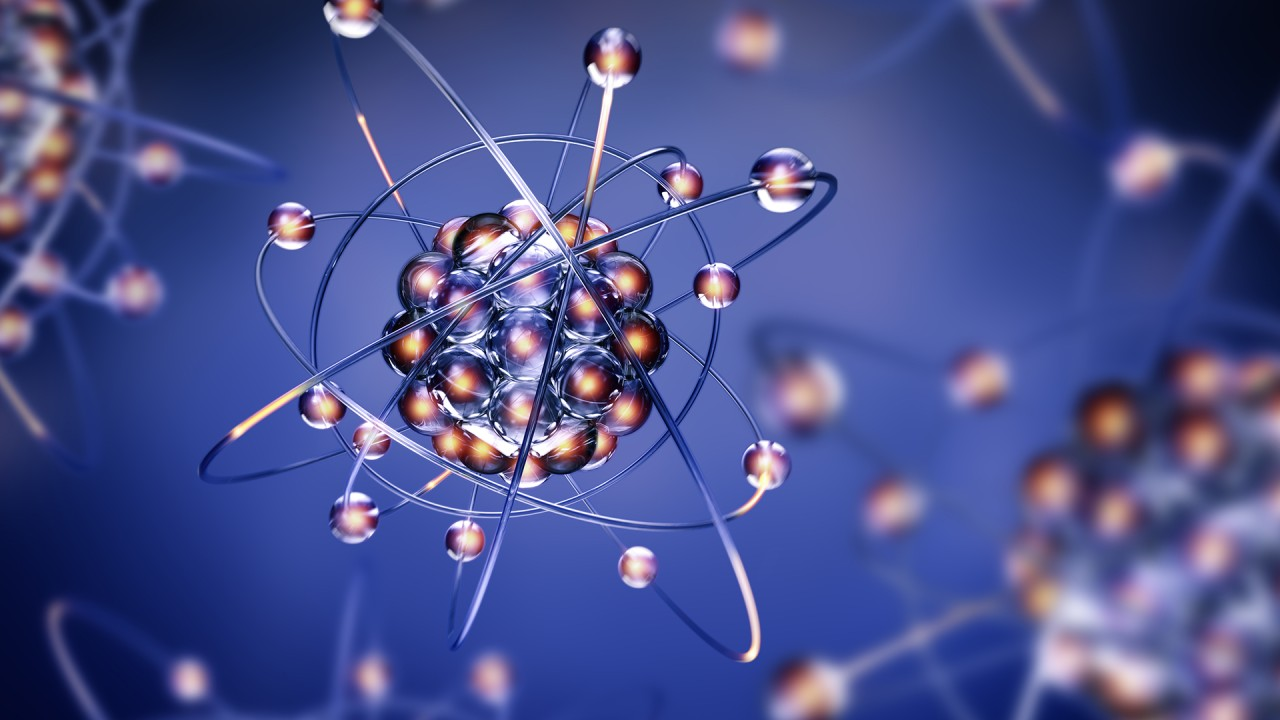
\includegraphics[width=\textwidth, height=0.9\textheight, keepaspectratio]{atom.jpg}
        \figciteweburl{Bonn.19.08.2021}
        % \vspace{0.5cm}
        % \begin{quote}
        %{Stellen Sie sich vor, ...}
        % \end{quote}
    \end{frame}

    % Title Slide
    \begin{frame}[noframenumbering, plain]
        \vspace*{-0.6cm}
        \titlepage
        \vspace*{-1.6cm}
    \end{frame}
    
    % Table of Contents
    \begin{frame}<handout:0>{Gliederung} % Handout ausgeschaltet!!
      \setcounter{page}{1}      
        \tableofcontents
    \end{frame}
    
    \section{Section 1}
    \begin{frame}{Slide 1}
      \begin{figure}
        \centering
        \begin{minipage}{0.5\textwidth}
          \centering
          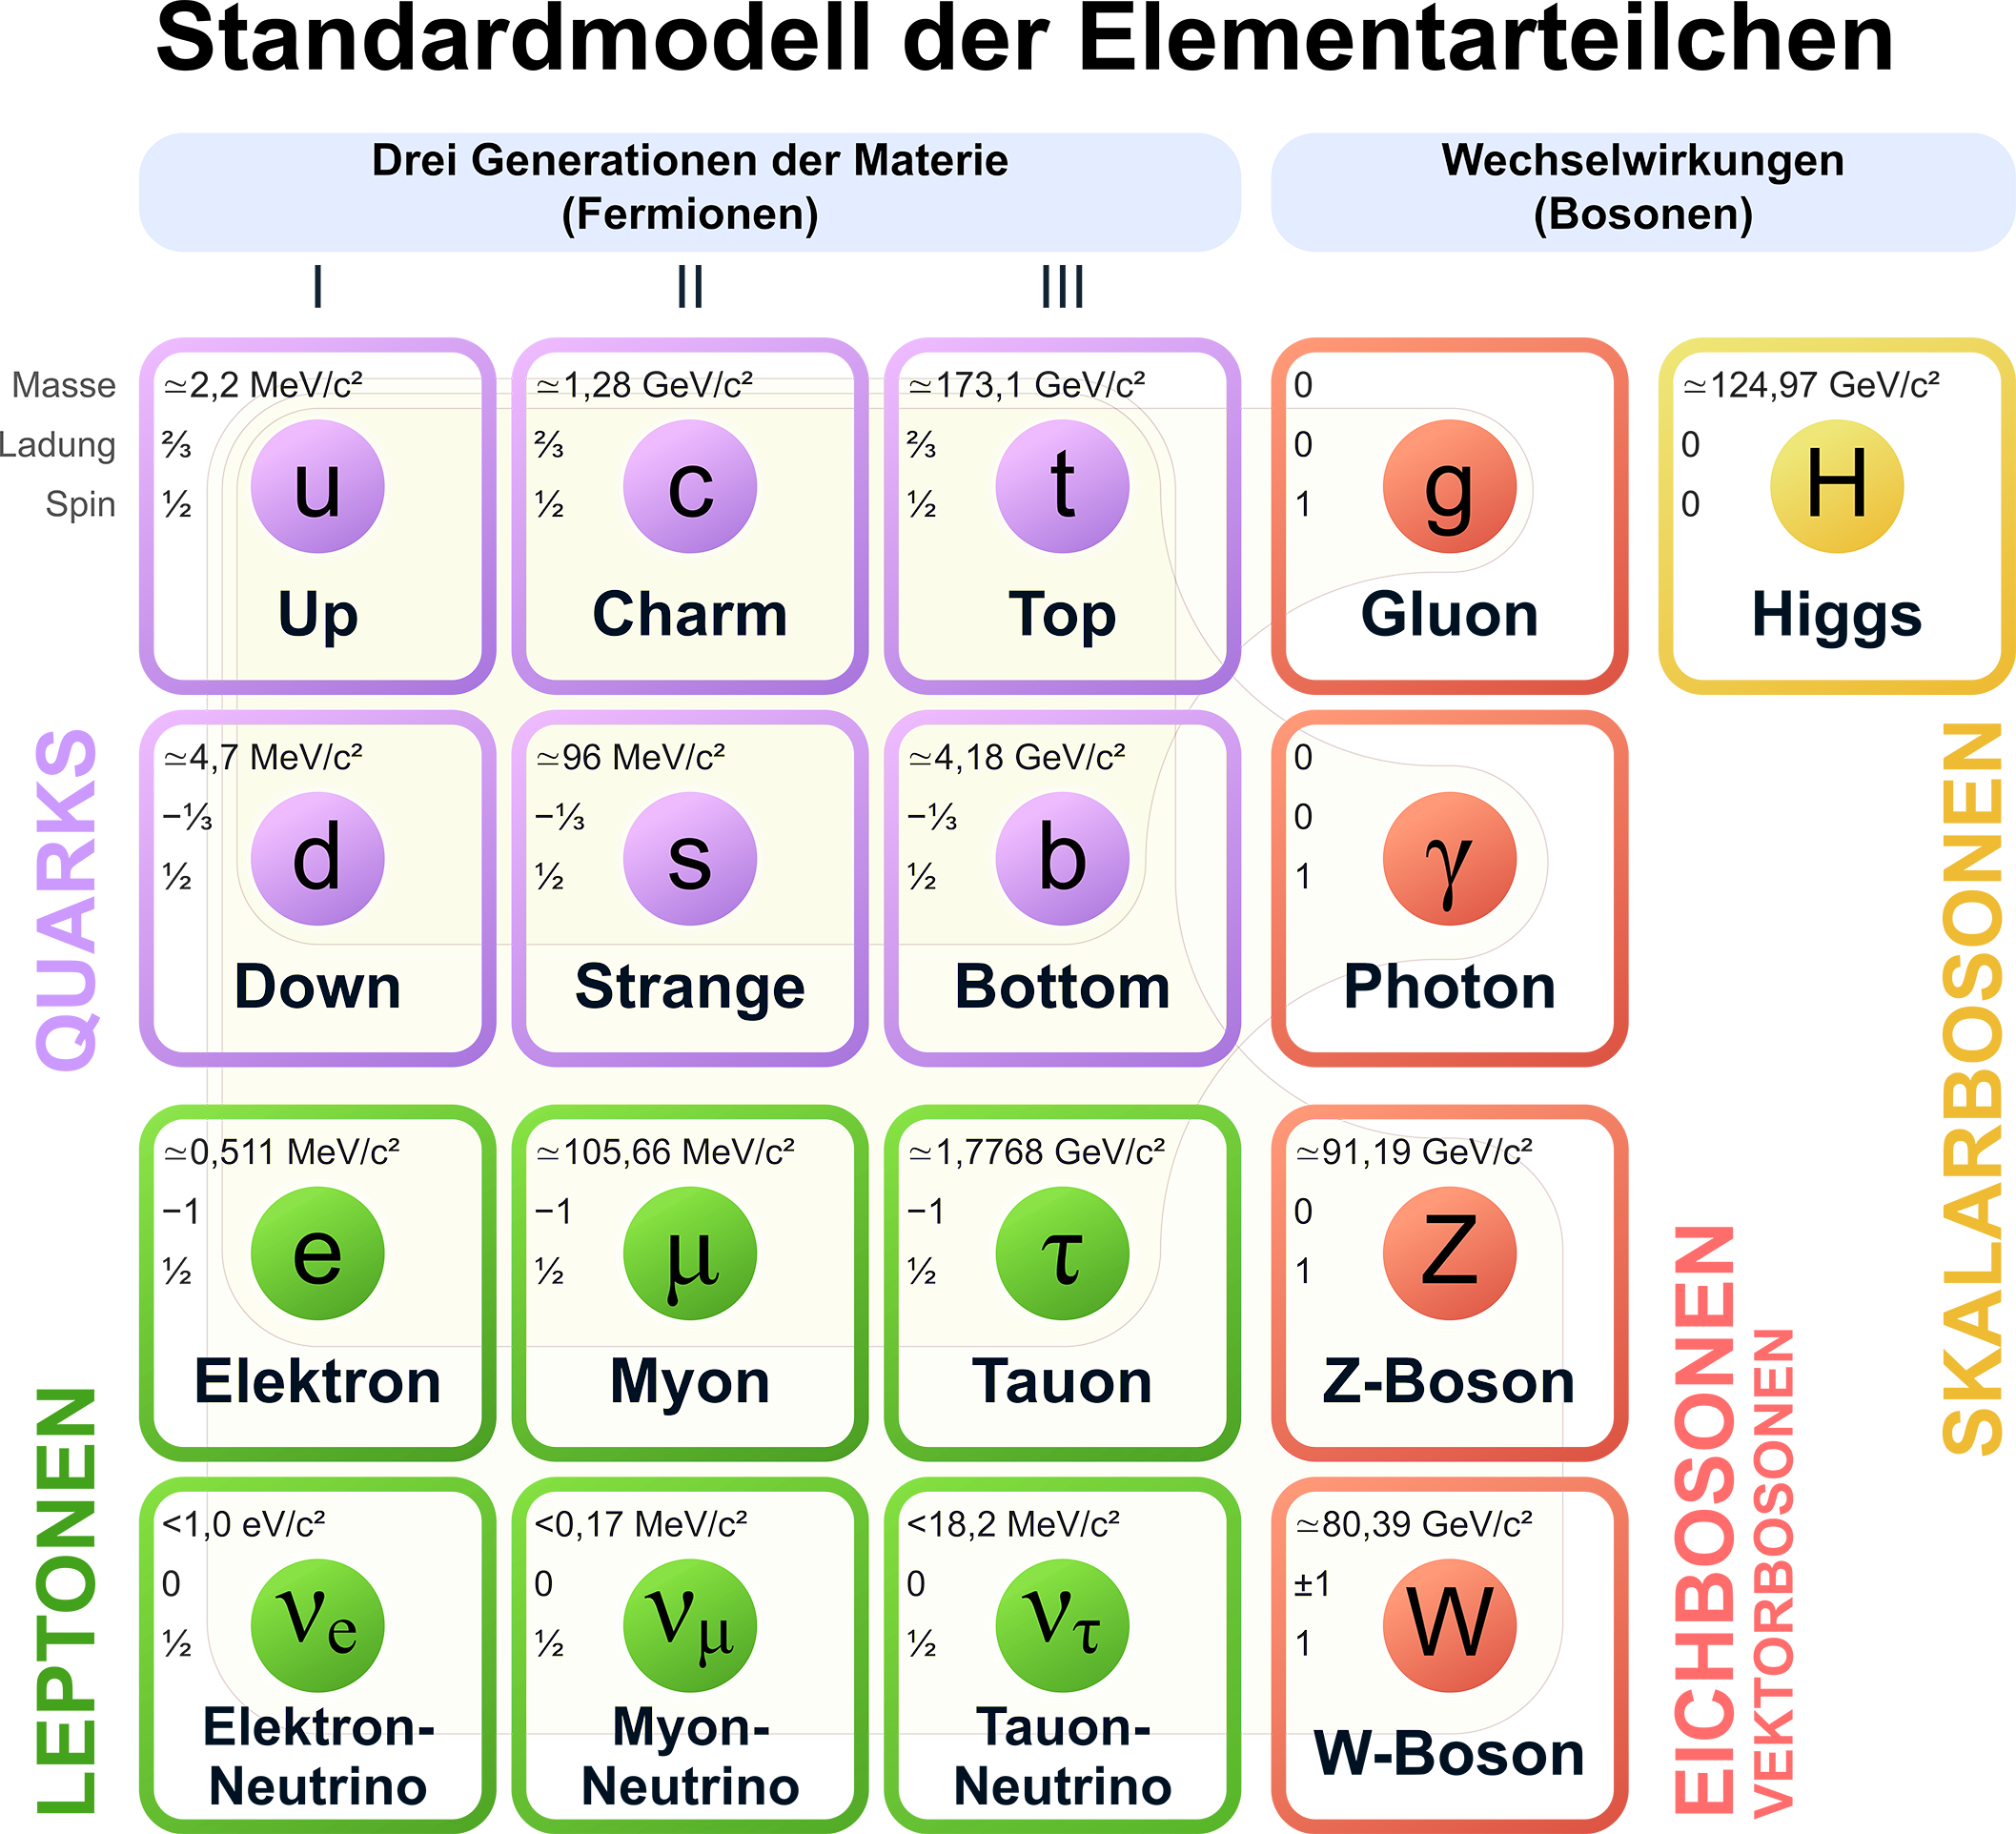
\includegraphics[width=\textwidth, keepaspectratio, height=0.85\textheight]{Standard_Model_of_Elementary_Particles_normal.png}\tiny
          \\\citeauthortitleurl{Wikipedia.Standardmodell}\end{minipage}
        \hfill \pause
        \begin{minipage}{0.48\textwidth}
          \begin{itemize}
            \item first point \pause
            \item second point \pause
            \item third point \pause
          \end{itemize}
          \end{minipage}
      \end{figure}
    \end{frame}

    \subsection{subsection 1}
    \begin{frame}{Slide 2}
      \begin{figure}
        \centering
        \begin{minipage}{0.5\textwidth}
          \centering
          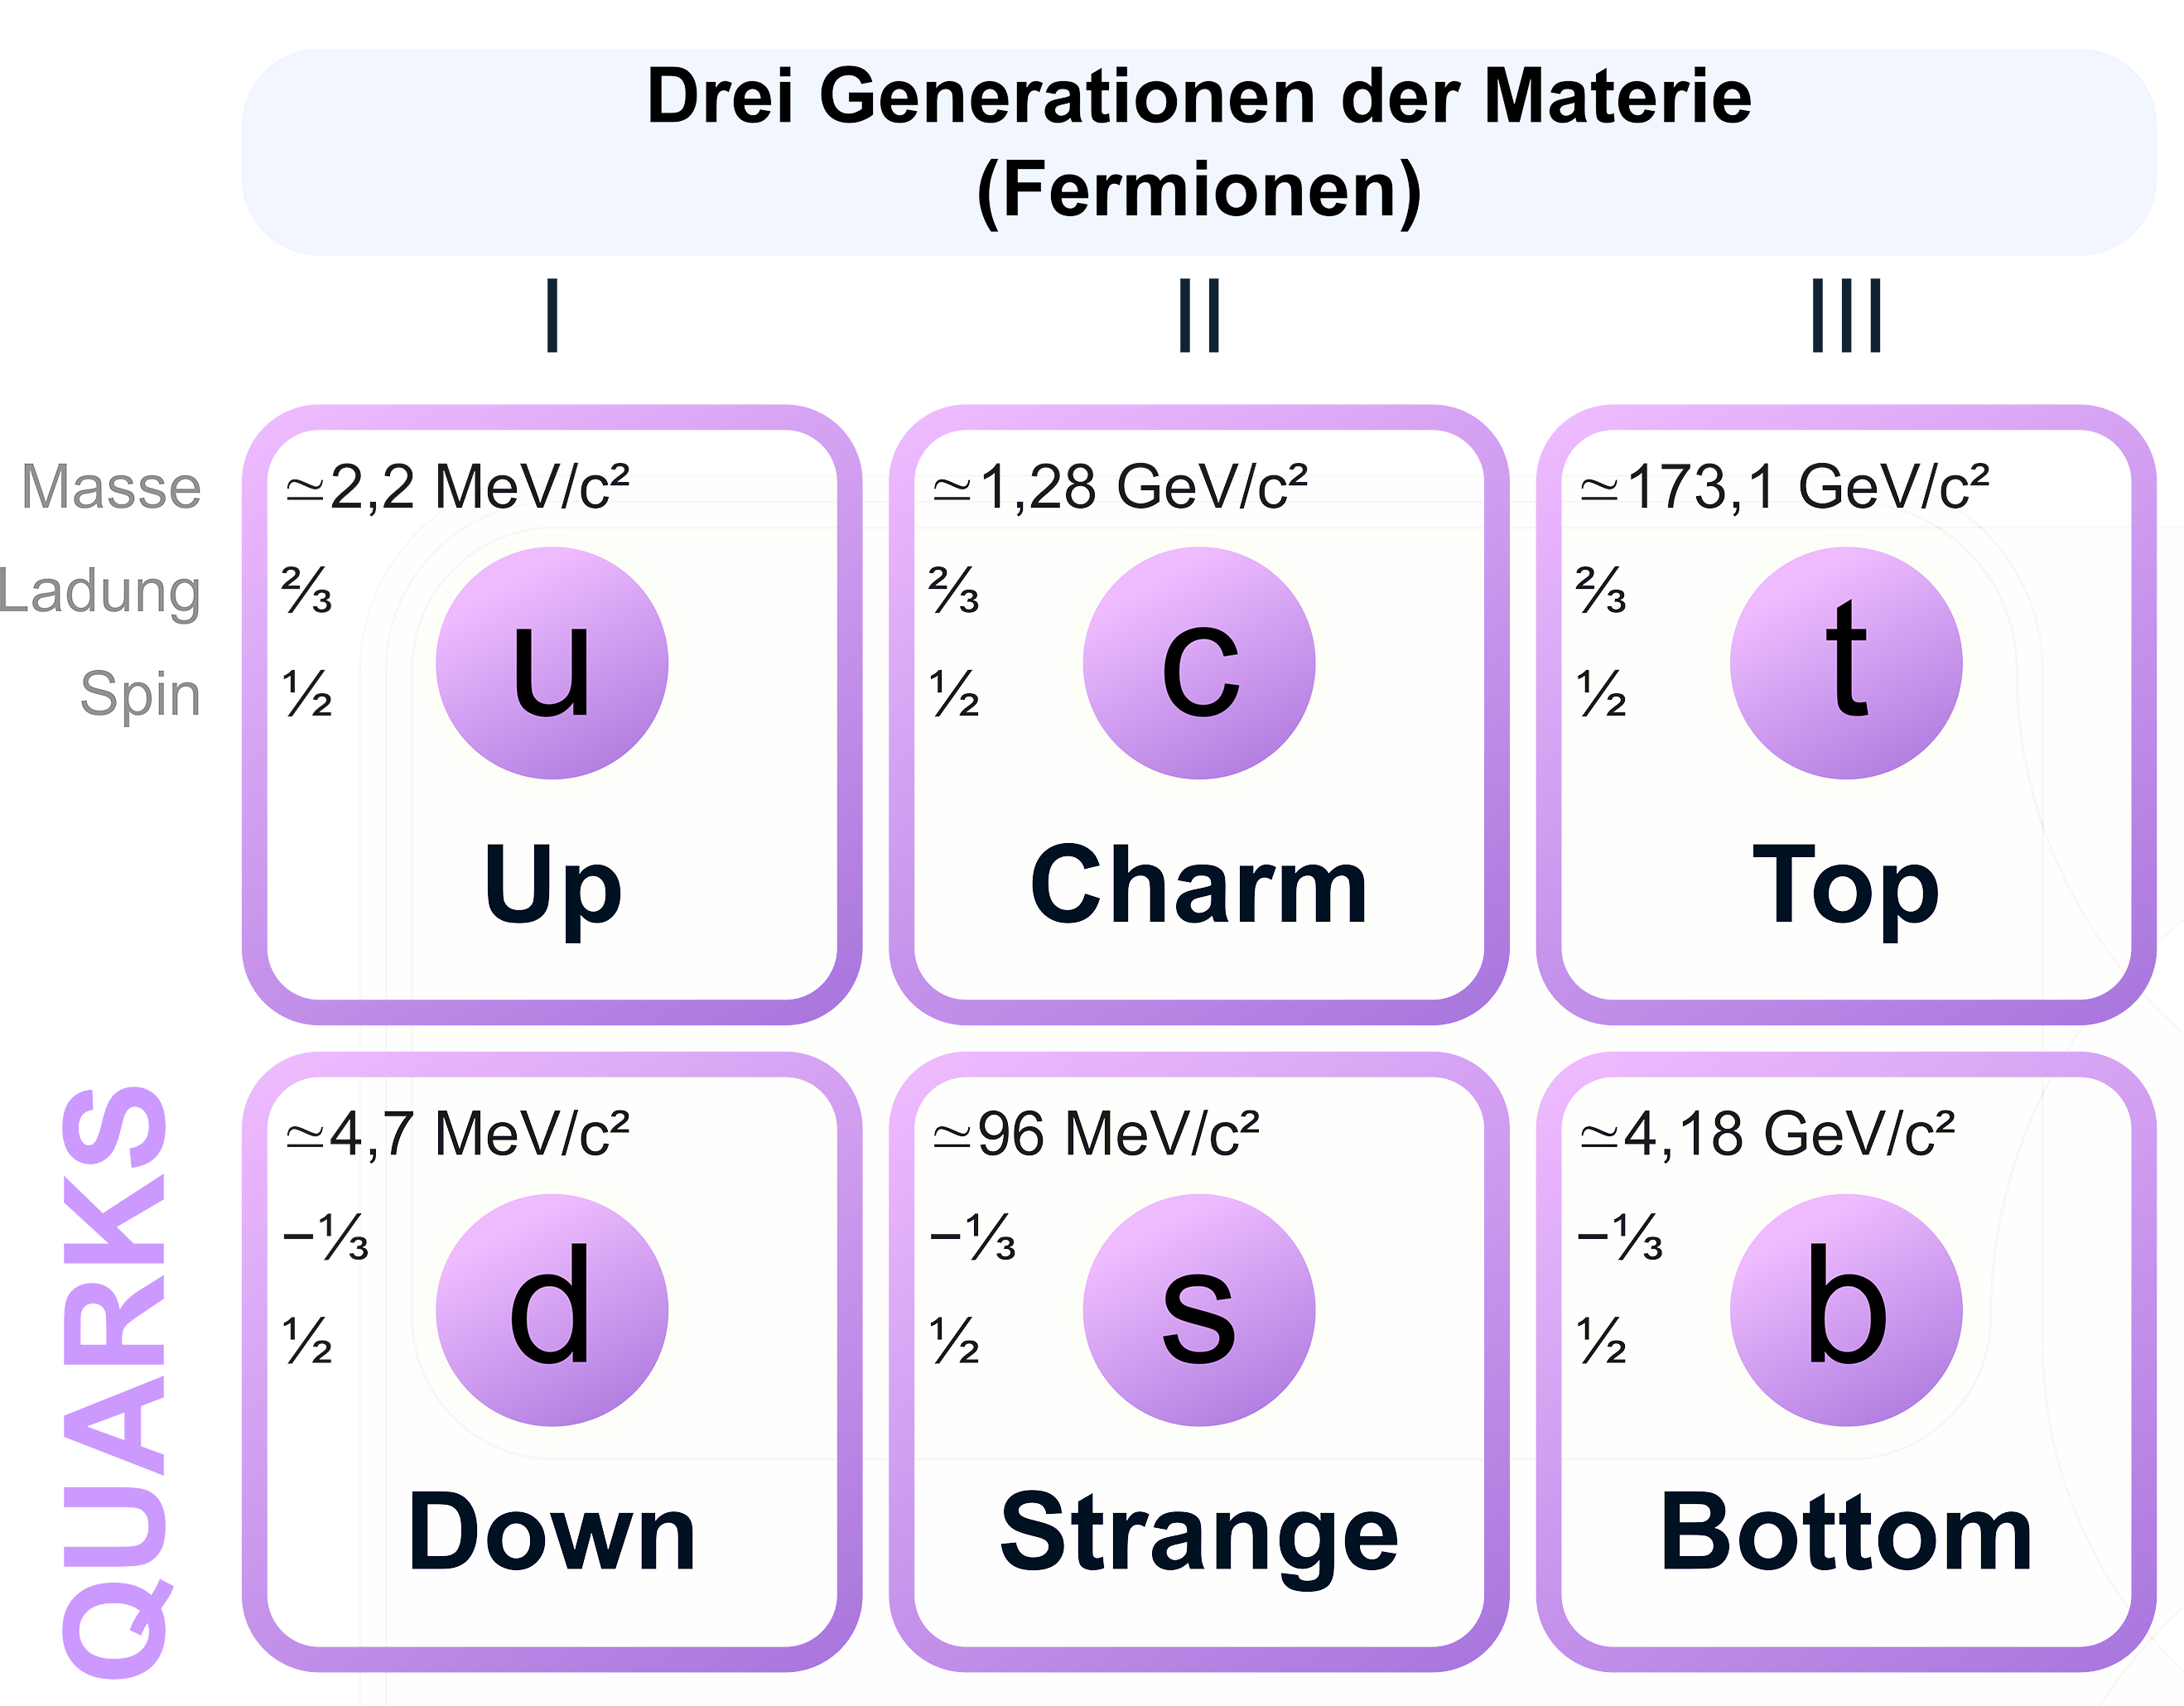
\includegraphics[width=\linewidth, keepaspectratio, height=\textheight]{Standard_Model_of_Elementary_Particles_zoom2.png}\tiny
          \\\citeauthortitleurl{Wikipedia.Standardmodell} \end{minipage}
        \hfill
        \begin{minipage}{0.48\textwidth}
          \begin{itemize}\pause
            \item Point one\pause
            \item Point two\pause
            \item Point three\pause
            \item Point four
          \end{itemize}
          \end{minipage}
      \end{figure}
    \end{frame}
    
    \section{Section 2}
    \begin{frame}{Fazit}
        \begin{itemize}
            \item Point one \pause
            \item Point two \pause
            \item Point three \pause
            \item Point four
        \end{itemize}
      \centering
      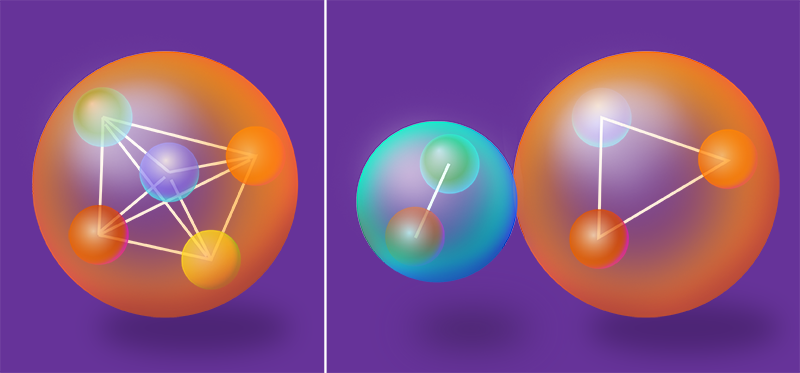
\includegraphics[width=\linewidth, height=0.46\textheight, keepaspectratio]{pentaquark model.png}
      \figciteweburl{KennethHicks.2015}
    \end{frame}

    % Thank You Slide
    \begin{frame}<handout:0>{Thank you for your attention!}
      \begin{center}
        \Huge Questions?
      \end{center}
  \end{frame}

% Black slide
\begin{frame}<handout:0>[plain, noframenumbering]
  \begin{tikzpicture}[remember picture, overlay]
      \fill[black] (current page.south west) rectangle (current page.north east);
  \end{tikzpicture}
\end{frame}

  \begin{frame}<handout:0>[noframenumbering, plain, allowframebreaks]{Anhang}
      \begin{minipage}{0.4\textwidth}
        \textbf{Quarkzusammensetzung}
        \begin{itemize}
          \item point one \pause
          \item point two \pause
          \item point three
        \end{itemize}
      \end{minipage}
      \hfill
      \begin{minipage}{0.58\textwidth}
        asfd
      \end{minipage}
      
    \pagebreak
      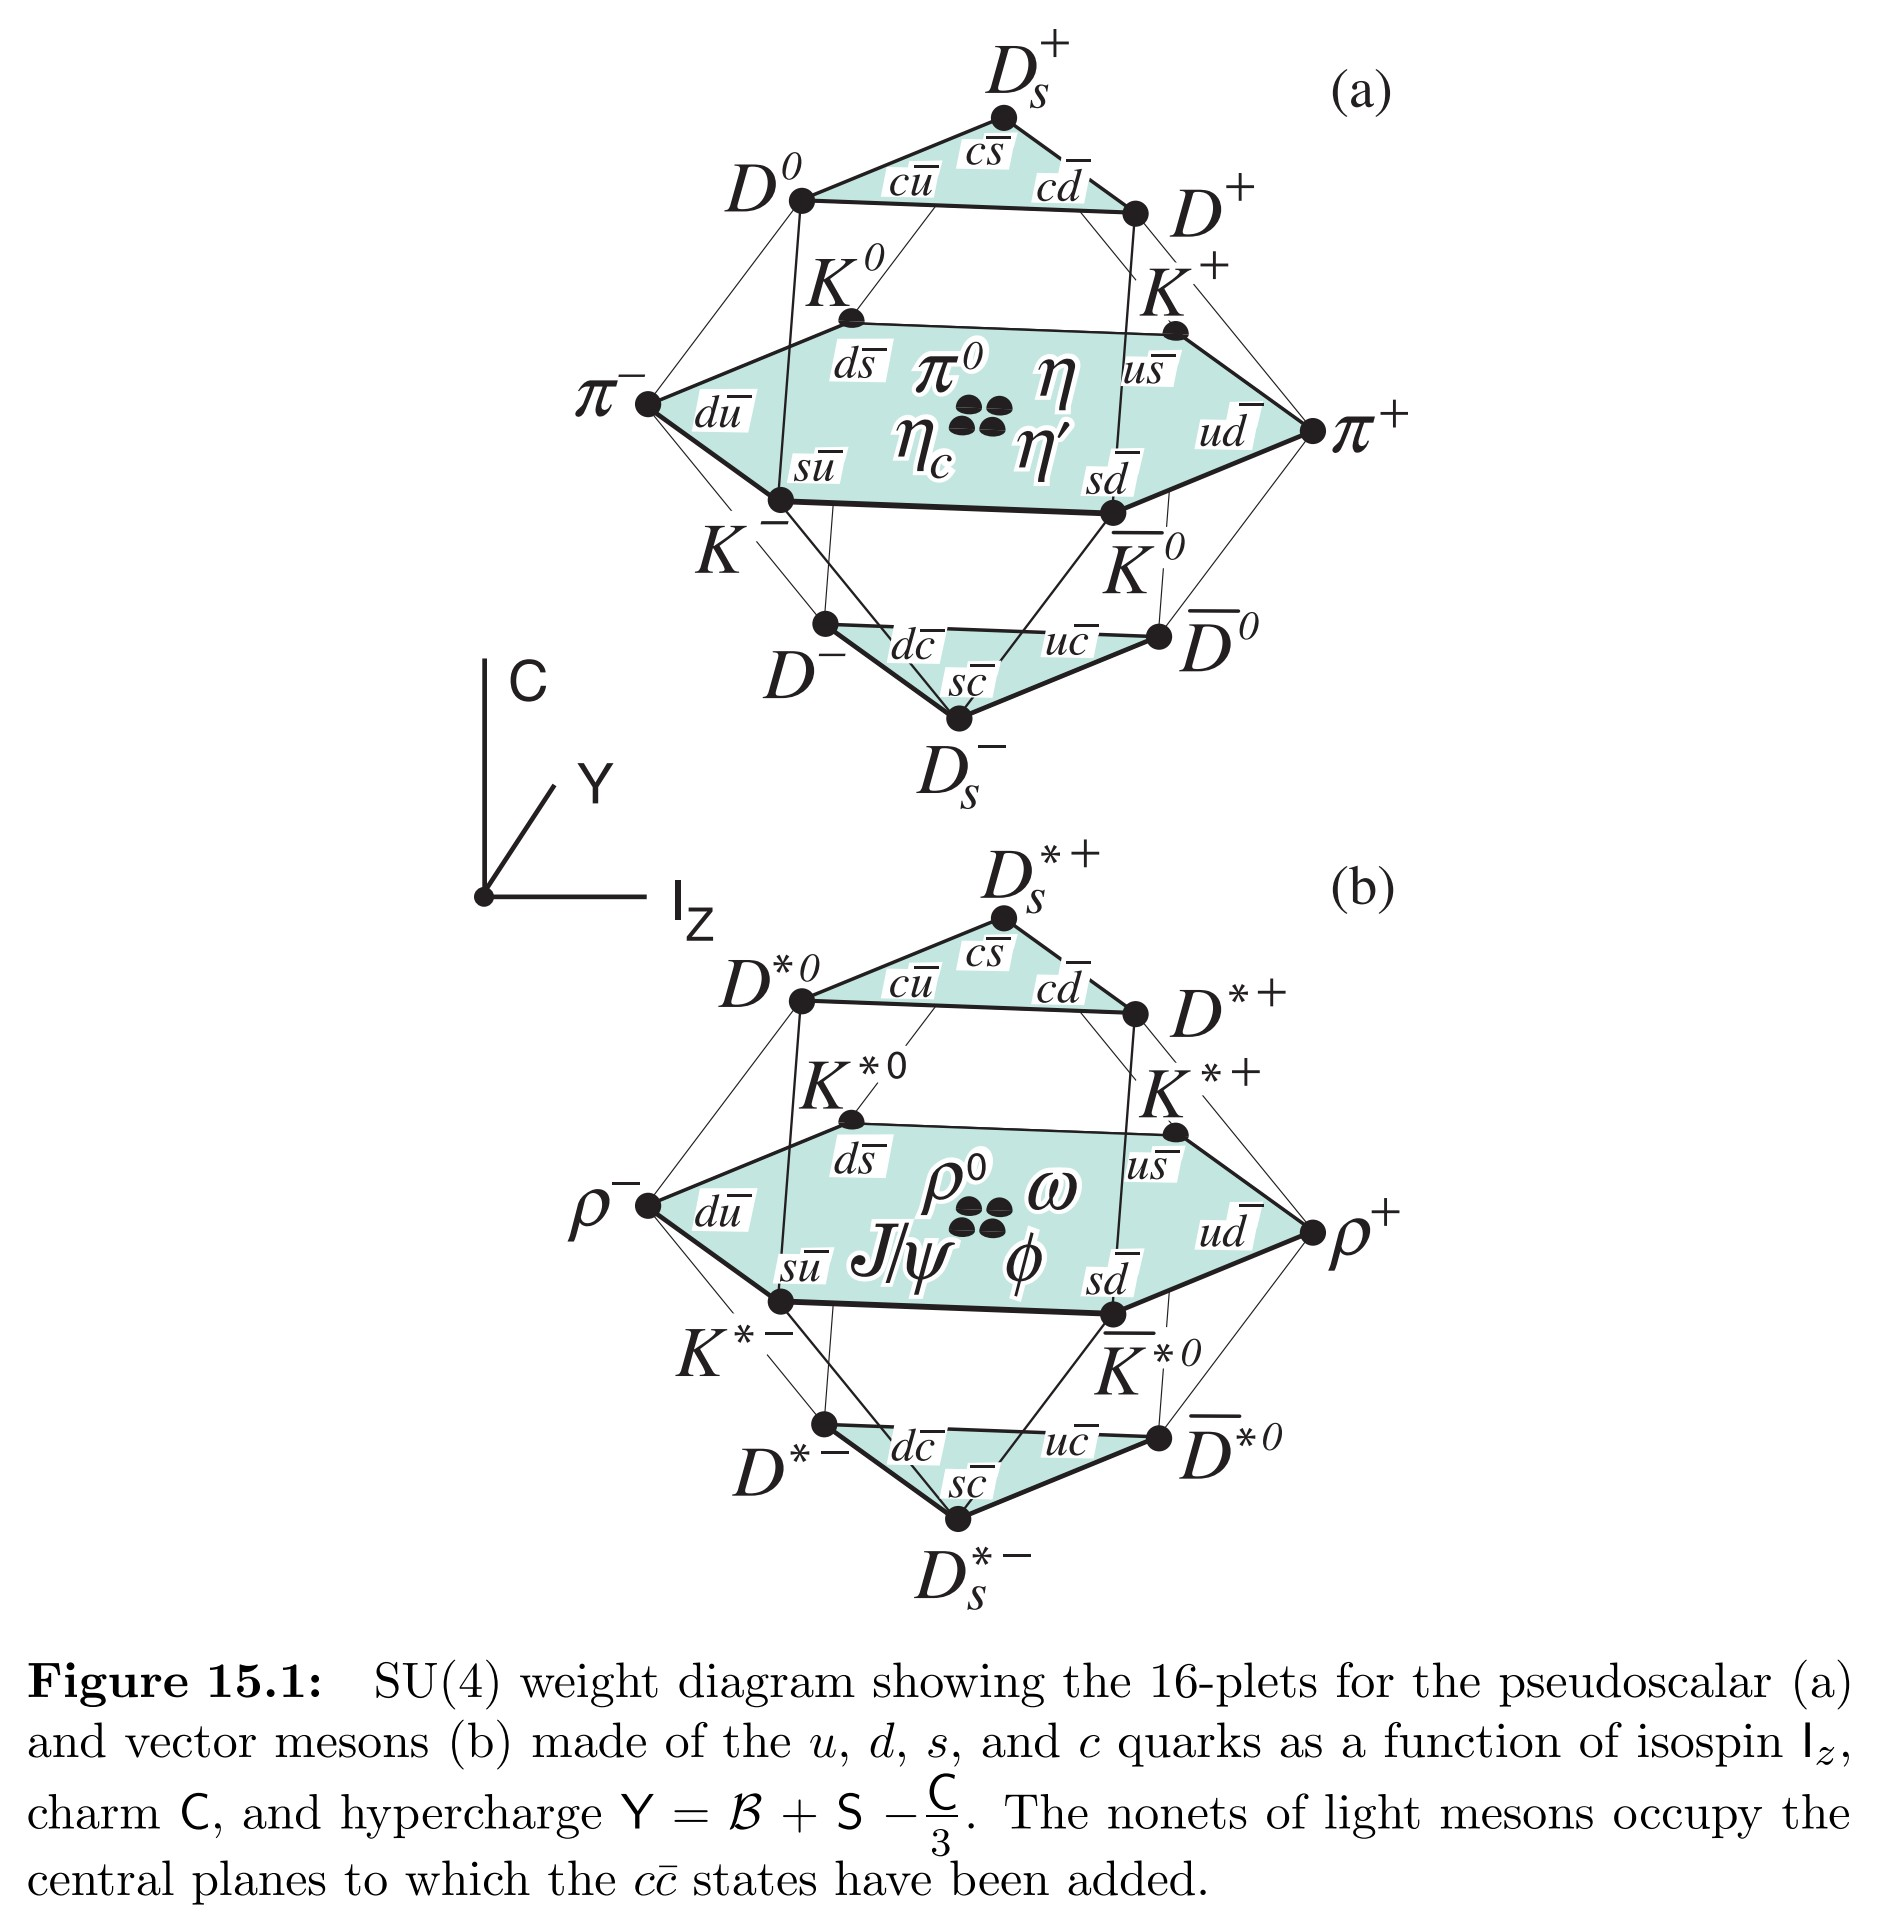
\includegraphics[height=0.9\textheight, width=\linewidth, keepaspectratio]{Images/90f0590a-0e4a-4d62-bd40-0bcce4be9feb.jpg}%\caption{C Amsler, T DeGrand et al 2017 - Quark Model.jpg}
      \figcite{C.Amsler.2017}
    
    \end{frame}


    
%     % Bibliography    
%     \begin{frame}[allowframebreaks, noframenumbering, plain]{Literaturverzeichnis}
%    \printbibliography%[nottype=unpublished]
%     \end{frame}

\end{document}
